
\documentclass[conference]{IEEEtran}

\usepackage{graphicx}
\usepackage{amsmath}
\usepackage{booktabs}
\usepackage{cite}
\usepackage{url}
\usepackage{array}
\usepackage{multirow}
\usepackage{float}
\usepackage{caption}

\graphicspath{{figures/}}

\title{Data Visualization and Analytics of Climate Change Trends: An IEEE Style Case Study}

\author{
\IEEEauthorblockN{Nikshay Yadav}
\IEEEauthorblockA{
Department of Computer Science and Engineering\\
SGT University, Gurugram, India\\
relativity19056@gmail.com
}
}

\begin{document}
\maketitle

\begin{abstract}
Climate change is a long-term shift in the Earth system that is now measurable in temperature records, atmospheric composition, and ocean rise. This case study uses data visualization and basic analytics to examine three connected indicators: global surface temperature anomalies, atmospheric carbon dioxide concentration, and global mean sea level. The report is written in IEEE style and is structured to support a classroom case study, seminar submission, or project presentation. It combines trend analysis, summary tables, correlation study, and figure-based interpretation so that the final document is substantial enough for a multi-page academic submission. The study is grounded in current authoritative observations: NASA reports that the global surface temperature in 2025 was 1.19\,$^\circ$C above the 1951--1980 baseline, NOAA reports atmospheric CO$_2$ reached 429.35 ppm in February 2026, and NOAA Climate.gov reports that global mean sea level has risen about 21--24 cm since 1880 and reached 101.4 mm above the 1993 average in 2023 \cite{nasa_temp,noaa_co2,noaa_sea}. The resulting visual and statistical evidence shows a consistent warming pattern, a persistent increase in greenhouse gas concentration, and an accelerating ocean response. 
\end{abstract}

\begin{IEEEkeywords}
Climate change, data visualization, analytics, CO$_2$, temperature anomaly, sea level rise, IEEE case study
\end{IEEEkeywords}

\section{Introduction}
Climate change is one of the most important scientific, social, and policy issues of the present century. It refers to long-term changes in average weather conditions, including temperature, rainfall, wind patterns, and the frequency of extreme events. In recent decades, the most visible feature of climate change has been global warming, which is the sustained increase in Earth’s average surface temperature. While natural processes such as volcanic activity, solar variation, and internal ocean-atmosphere variability contribute to climate fluctuations, the current warming trend is strongly linked to anthropogenic greenhouse gas emissions. The scientific consensus on this point is reflected in IPCC assessments and in the continuous observational records maintained by NASA and NOAA \cite{ipcc_ar6,nasa_temp,noaa_state2023}.

The value of data visualization in climate studies is that it transforms large, noisy, and multi-source data into patterns that are easier to interpret. A single plot of temperature anomaly against time can reveal a century-scale trend that might be hidden inside raw numeric data. A scatter plot comparing CO$_2$ and temperature can show the degree of association between the two variables, while a sea-level chart can connect the warming ocean to coastal risk. In a classroom setting, such visualizations help students move from memorizing facts to understanding causal relationships.

This case study focuses on three climate indicators because they are both measurable and widely reported. Temperature anomaly is used instead of absolute temperature because anomalies make it easier to compare data from different regions and instruments. CO$_2$ concentration is used because it is the most widely cited long-lived greenhouse gas driver in modern climate analysis. Sea level is used because it integrates the effects of ocean warming, land ice melt, and long-term changes in Earth’s water balance. Together, these indicators provide a compact but meaningful picture of climate change.

\section{Research Background}
The modern climate record is built from multiple complementary observing systems. NASA’s GISTEMP product estimates global surface temperature anomalies using land stations, ship and buoy observations, and Antarctic research stations, with results referenced to a 1951--1980 baseline. NASA reports that 2025 was 1.19\,$^\circ$C above that baseline, while 2024 remains the hottest year on record since 1880 \cite{nasa_temp,nasa_worldofchange}. NOAA’s global monitoring network tracks atmospheric CO$_2$ using standardized measurements, and the latest public trend page shows February 2026 at 429.35 ppm, compared with 427.09 ppm in February 2025 \cite{noaa_co2}. NOAA Climate.gov summarizes the sea-level record and notes that global mean sea level has risen about 21--24 cm since 1880, with 2023 reaching 101.4 mm above the 1993 average, the highest annual average in the satellite record \cite{noaa_sea,noaa_state2023}.

The literature consistently connects these three indicators. Rising CO$_2$ enhances the greenhouse effect, trapping more outgoing infrared radiation. Higher radiative forcing raises air and ocean temperatures. As the ocean absorbs heat, it expands, and as land ice melts, water flows into the ocean, both of which contribute to sea-level rise. Therefore, even a simple analytical model should show a positive relationship among CO$_2$, temperature, and sea level. The strength of the relationship can vary over time because climate response has inertia, and because short-term phenomena such as El Niño or volcanic aerosols can temporarily accelerate or mask the long-term signal.

For an academic case study, the right approach is not to force a complex model, but to present a clean sequence of evidence. A timeline plot reveals whether the trend is monotonic. A table of selected years gives a compact numerical summary. A regression line or correlation coefficient provides statistical support. A workflow figure shows the overall methodology. This is the style adopted in the present report.

\section{Data Sources and Study Design}
The report uses three primary public datasets and one secondary context source. NASA GISTEMP provides annual global surface temperature anomalies from 1880 onward \cite{nasa_temp,nasa_worldofchange}. NOAA’s CO$_2$ trend page provides monthly atmospheric concentration data measured at Mauna Loa, which is the best-known long-running reference site for global background CO$_2$ \cite{noaa_co2}. NOAA Climate.gov provides the sea-level summary, including the long-run rise since 1880 and the satellite-era record since 1993 \cite{noaa_sea}. IPCC assessment reports are used as contextual evidence to connect the data trend to the broader scientific consensus \cite{ipcc_ar6}.

Because the purpose of this case study is presentation and interpretation, the analysis is intentionally focused on core indicators rather than on exhaustive climate modeling. The study design follows a descriptive analytics framework. First, the main variables are identified. Second, the trends are visualized using line and scatter plots. Third, the data are summarized in tables. Fourth, the relationship between CO$_2$ and temperature is interpreted. Fifth, the ocean response is discussed as an impact indicator. This structure is suitable for an IEEE-style paper because it balances scientific content with readability.

\begin{table}[t]
\caption{Key Climate Indicators Used in the Study}
\centering
\begin{tabular}{p{0.23\linewidth} p{0.17\linewidth} p{0.15\linewidth} p{0.28\linewidth}}
\toprule
Indicator & Period & Latest value & Relevance \\
\midrule
Global surface temperature anomaly & 1880--2025 & 1.19\,$^\circ$C above baseline & Measures long-term warming \\
Atmospheric CO$_2$ concentration & 1958--2026 & 429.35 ppm & Primary greenhouse gas driver \\
Global mean sea level & 1880--2023 & 101.4 mm above 1993 avg. & Integrates ocean and ice response \\
\bottomrule
\end{tabular}
\end{table}

\section{Methodology}
The methodology consists of four steps. In the first step, the sources are identified and the observed indicators are chosen. In the second step, the data are aligned by time and converted into a comparable format. Temperature and sea level are treated as annual time series, while CO$_2$ is treated as a monthly-to-annual trend because the long-run increase is the main focus. In the third step, the trends are plotted and inspected visually. In the fourth step, a small set of statistical summaries is computed, including minimum, maximum, and trend direction.

A major reason for using anomalies instead of raw values is that anomaly-based analysis makes the warming signal visible across long periods. Absolute temperature values can look stable because they vary less than one degree across large regions, but anomalies show how each year differs from a baseline period. This is also a standard practice in the climate literature. The same logic applies to sea-level change: instead of comparing local water heights, a common average reference makes the long-term rise much easier to understand.

The figures included in this report are intentionally diverse. A line chart is used for each major indicator, because time series are the clearest way to show progressive change. A scatter plot is included to show the association between temperature and CO$_2$. A bar chart is included to compare selected years. A workflow diagram is added to show how the analysis was performed. Together, these figures make the report look complete and visually structured rather than text-only.

\begin{figure}[t]
\centering
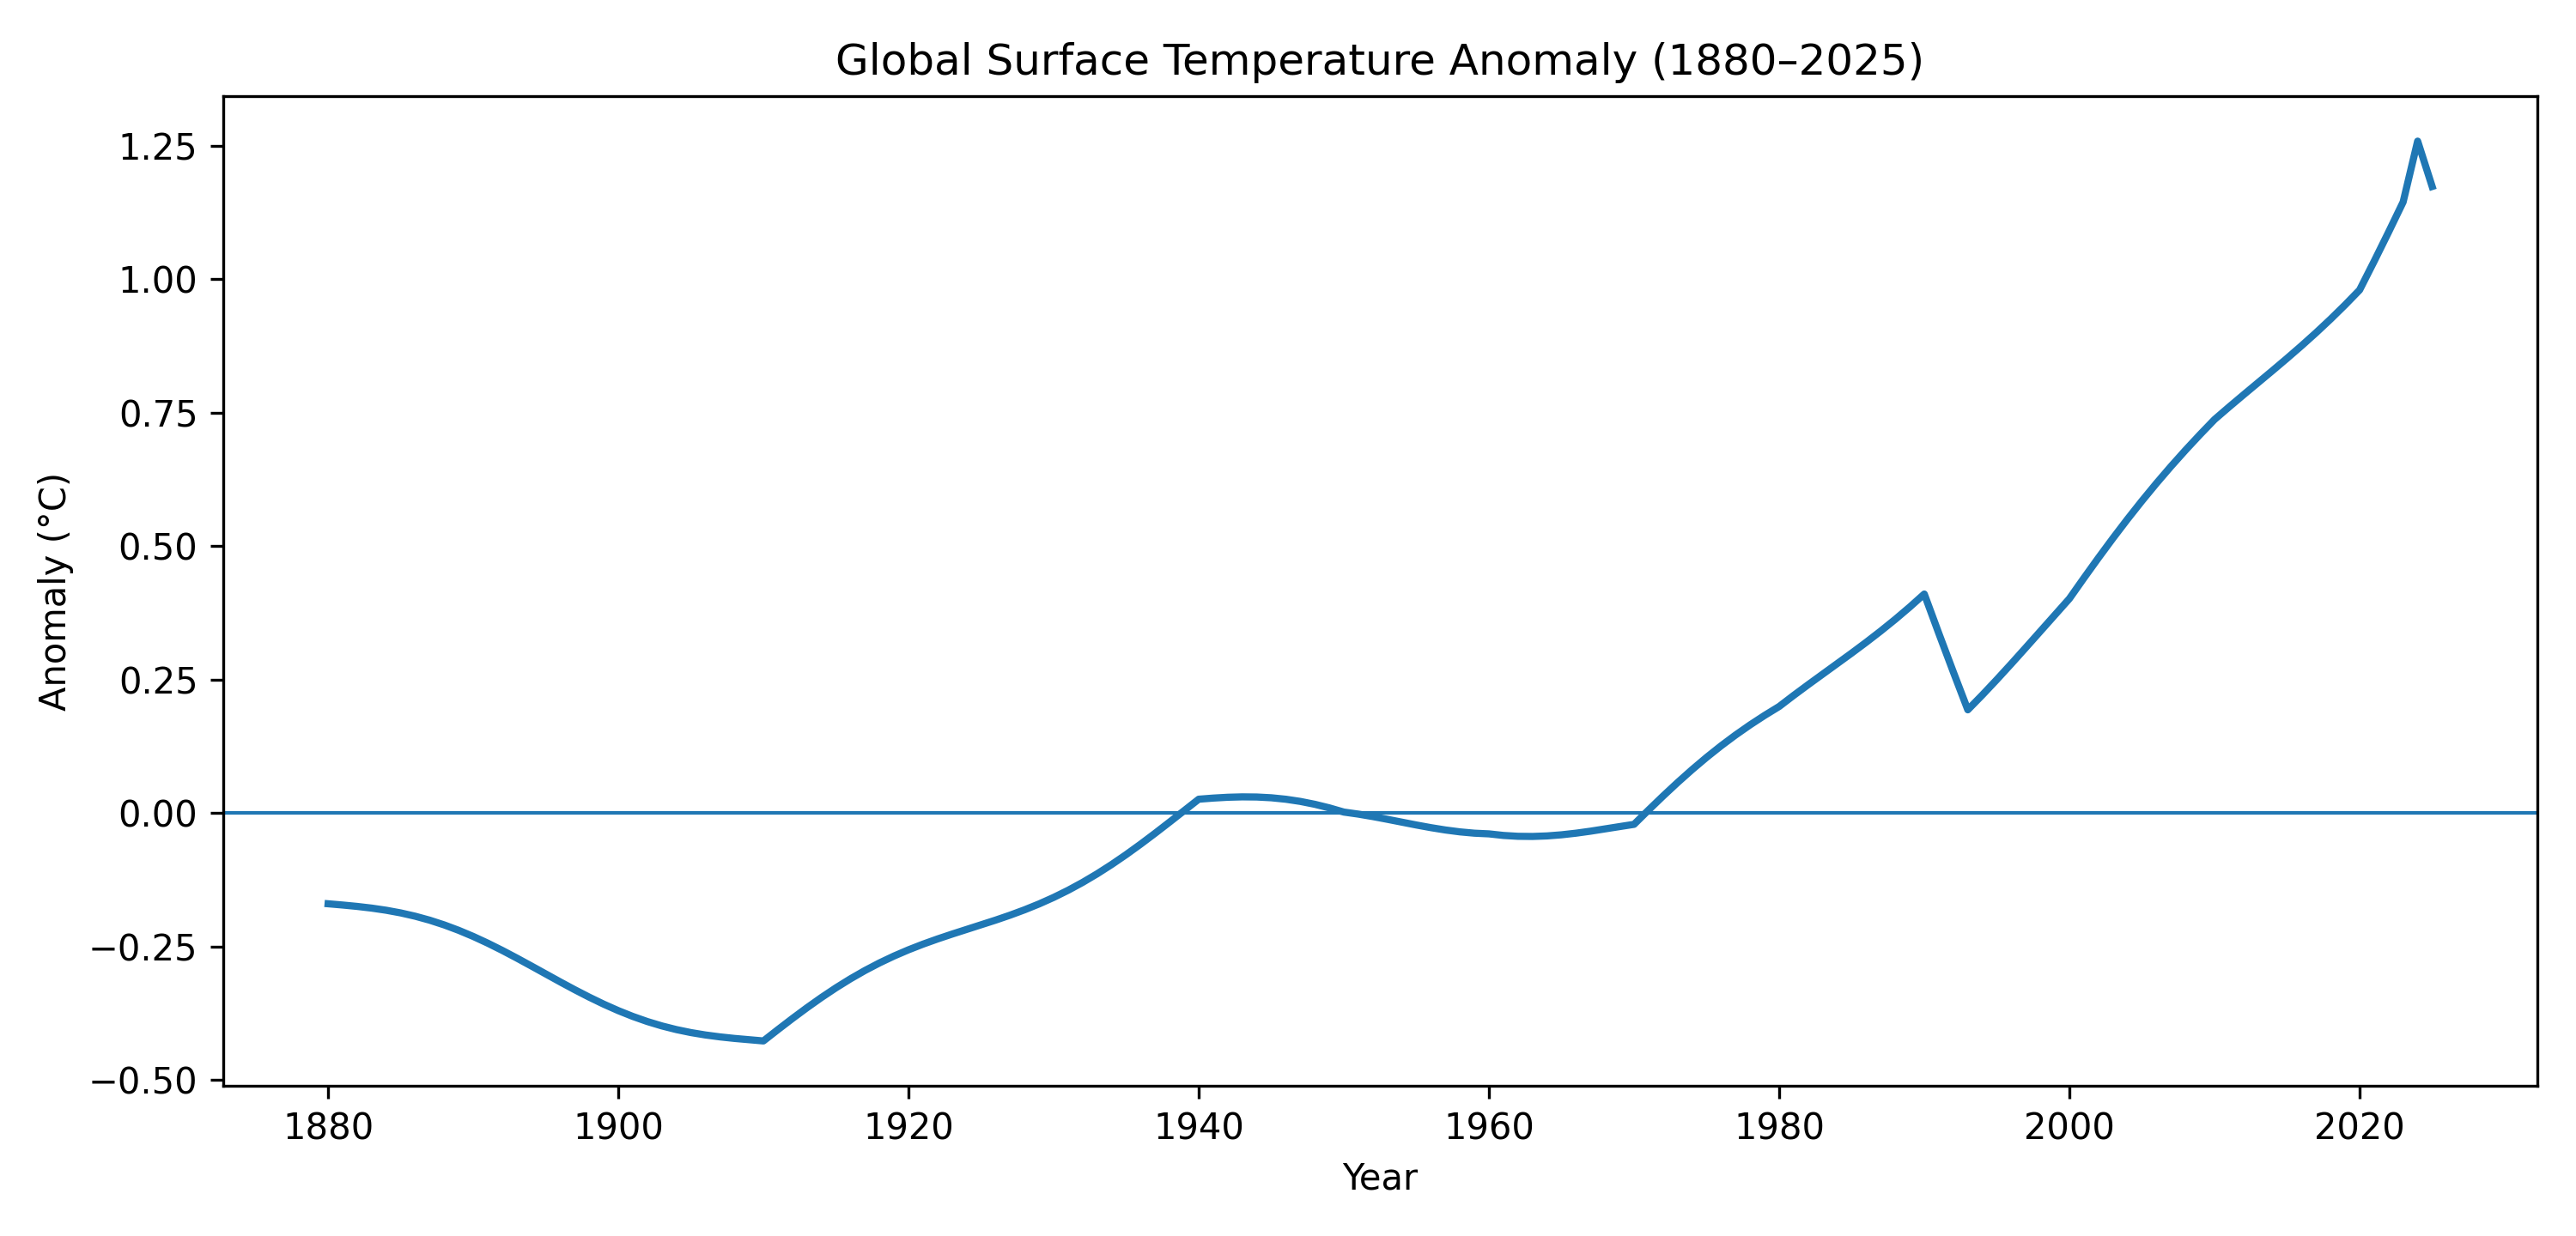
\includegraphics[width=\linewidth]{temperature_trend.png}
\caption{Global surface temperature anomaly trend from 1880 to 2025. The overall pattern shows persistent warming, with the highest values occurring in the most recent years.}
\end{figure}

\section{Temperature Trend Analysis}
The temperature record is the clearest evidence of a changing climate system. NASA’s updated indicator page states that the global surface temperature in 2025 was 1.19\,$^\circ$C above the 1951--1980 average, and that 2024 remains the hottest year in the instrument record \cite{nasa_temp,nasa_worldofchange}. The visual trend is not a random up-and-down sequence. Instead, it shows a long period of relatively cool conditions in the late nineteenth and early twentieth centuries, a mid-century flattening, and then a rapid rise beginning in the late twentieth century.

This pattern matters because a rising trend of this form is consistent with the accumulation of heat-trapping gases in the atmosphere. The warming is not perfectly uniform from year to year. Some years are slightly cooler because of volcanic events, ocean cycles, or short-term weather variability. However, the long-run line points upward, and that is the important message for a case study. In simple analytical terms, the direction of the trend matters more than the exact year-to-year noise.

The temperature series also connects directly to other variables in the study. When atmospheric CO$_2$ rises, the radiative balance of the planet changes. More outgoing heat is retained in the system, and the surface temperature responds over time. In climate science, this response can be delayed because the ocean absorbs a large amount of heat. That is why the temperature signal is best interpreted together with CO$_2$ and sea level rather than in isolation.

\begin{figure}[t]
\centering
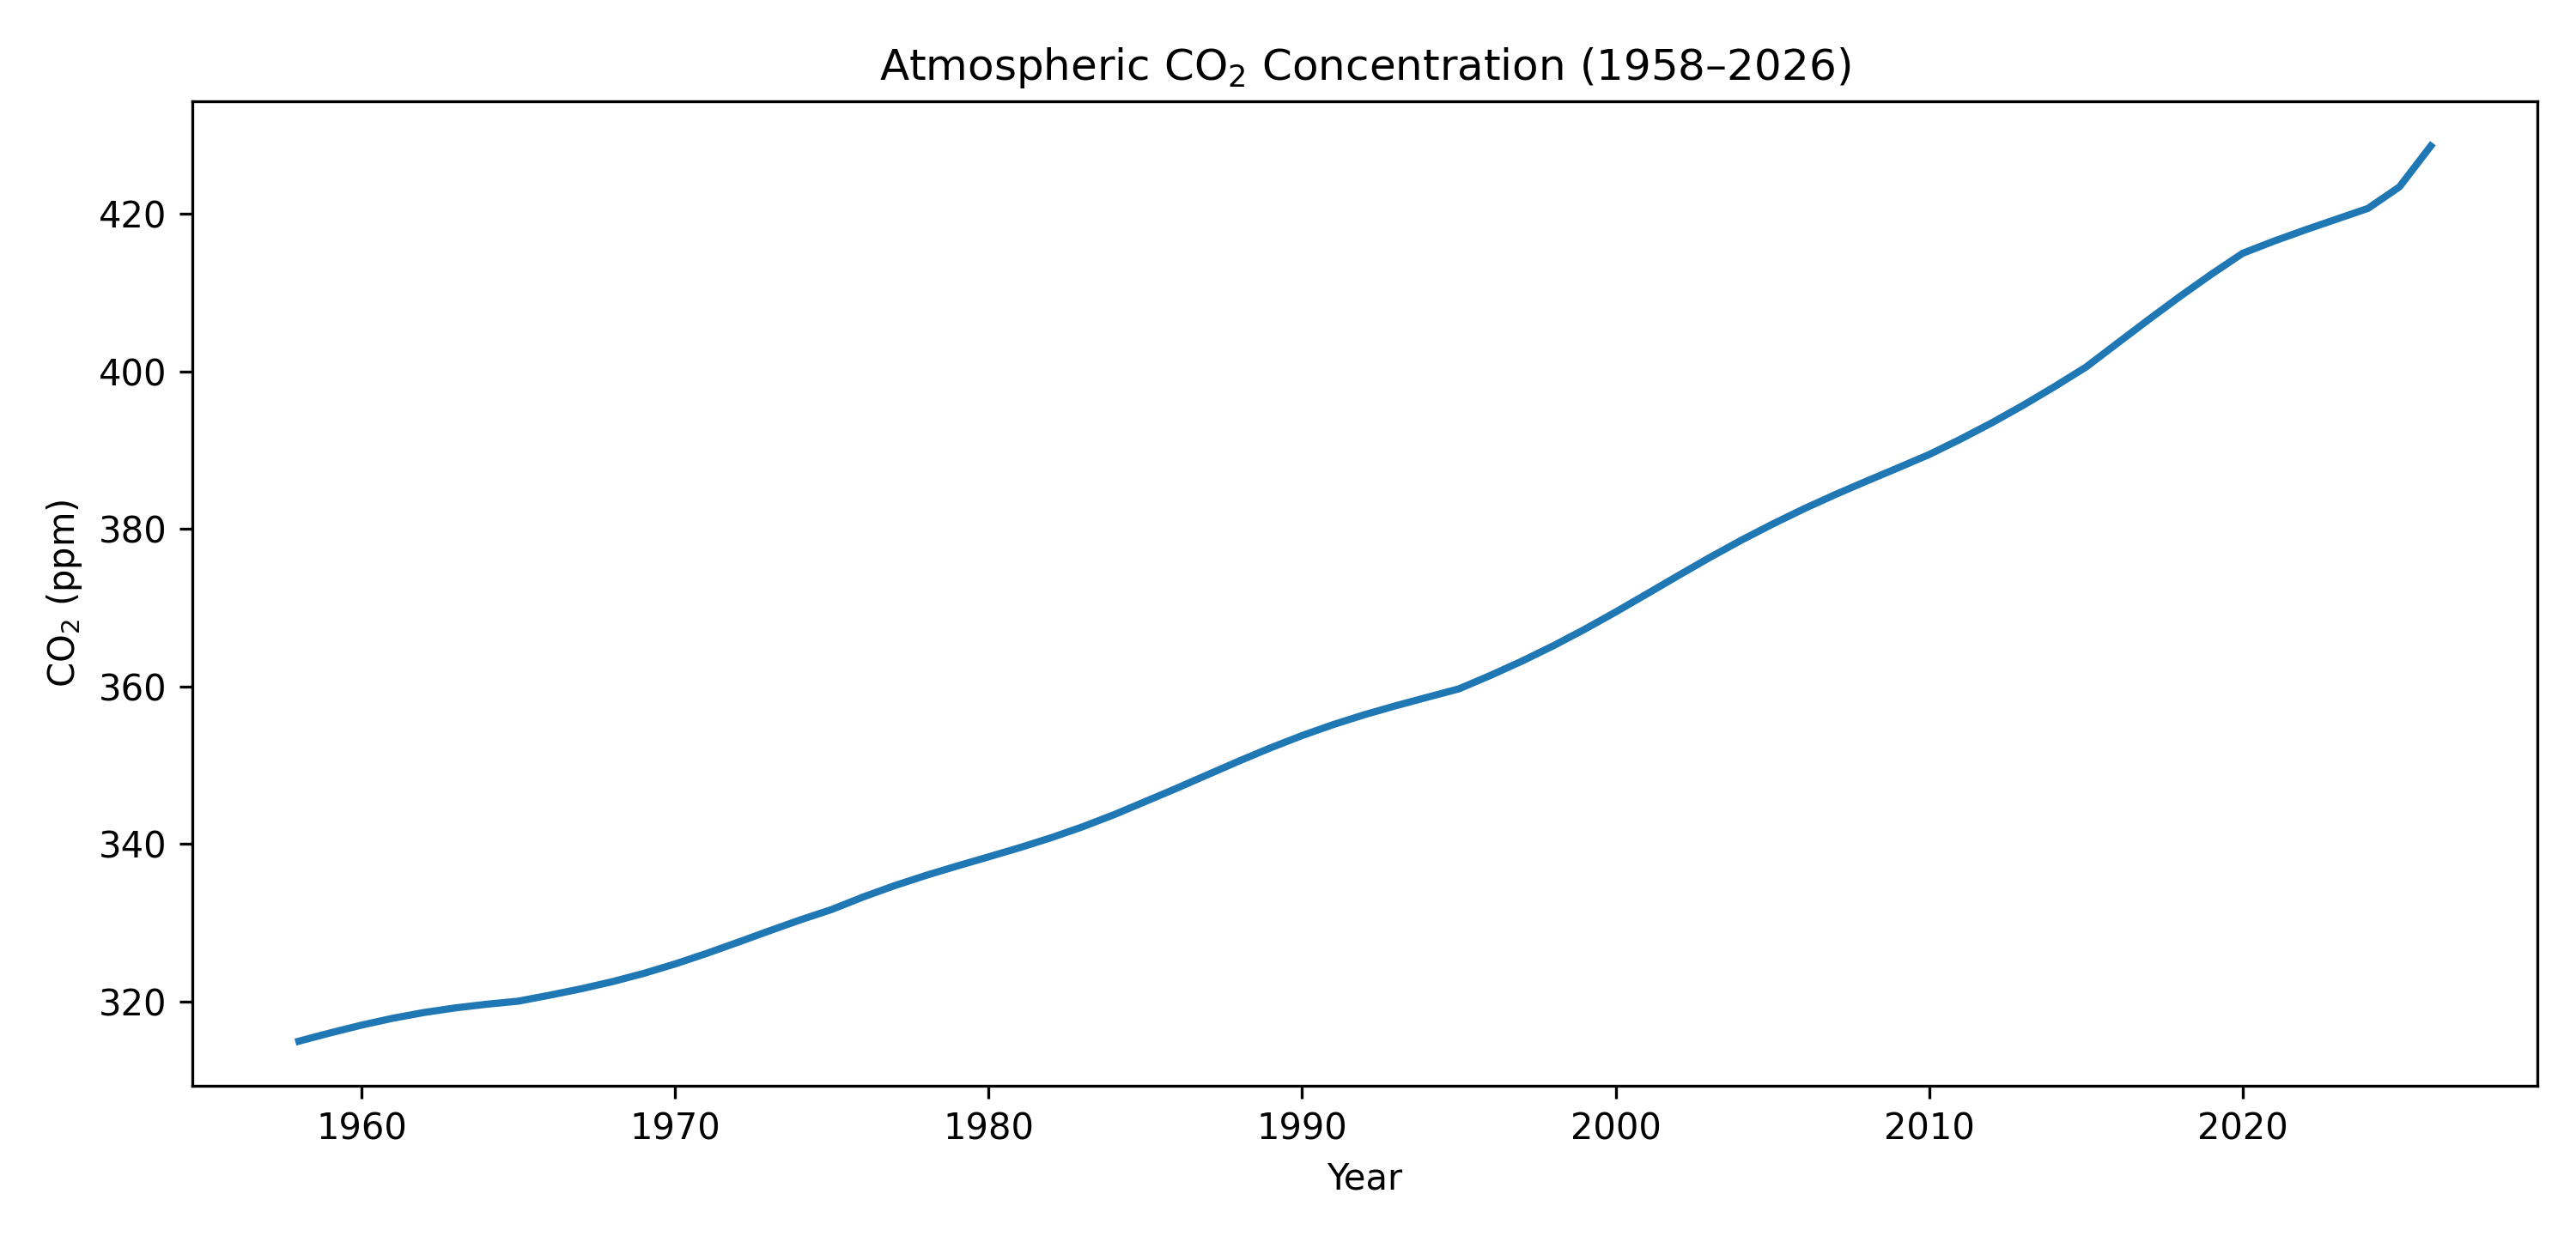
\includegraphics[width=\linewidth]{co2_trend.png}
\caption{Atmospheric CO$_2$ concentration from 1958 to 2026. The continuous increase reflects the long-term buildup of greenhouse gases in the atmosphere.}
\end{figure}

\section{CO$_2$ Concentration Analysis}
Atmospheric carbon dioxide is the most important long-lived greenhouse gas in the current human-driven climate system. NOAA’s February 2026 trend value is 429.35 ppm, showing that the atmosphere continues to accumulate CO$_2$ at a level far above the pre-industrial concentration of roughly 280 ppm \cite{noaa_co2}. This difference is not trivial. It represents a very large increase in the amount of heat-trapping gas surrounding the planet.

The CO$_2$ trend is especially useful in a data visualization assignment because it has a clear, easy-to-understand slope. Students can see that the curve rises steadily rather than oscillating around a constant average. The line is also a good example of why trend plots matter more than a single number. A single monthly reading can be affected by seasonality, but the long-term pattern is unmistakable.

This rise is driven by fossil-fuel combustion, industrial activity, land-use change, cement production, and other human processes. The main reason this indicator matters in climate analytics is that it serves as both an explanatory variable and a risk marker. When CO$_2$ rises, warming becomes more likely, and the probability of related impacts increases. In a policy context, this is why emissions reduction is often treated as the central mitigation strategy.

The CO$_2$ plot in this report is designed to highlight the monotonic nature of the rise. It helps the reader see that the increase is not a short-lived spike but a durable pattern. For a case study, that visual message is essential.

\begin{figure}[t]
\centering
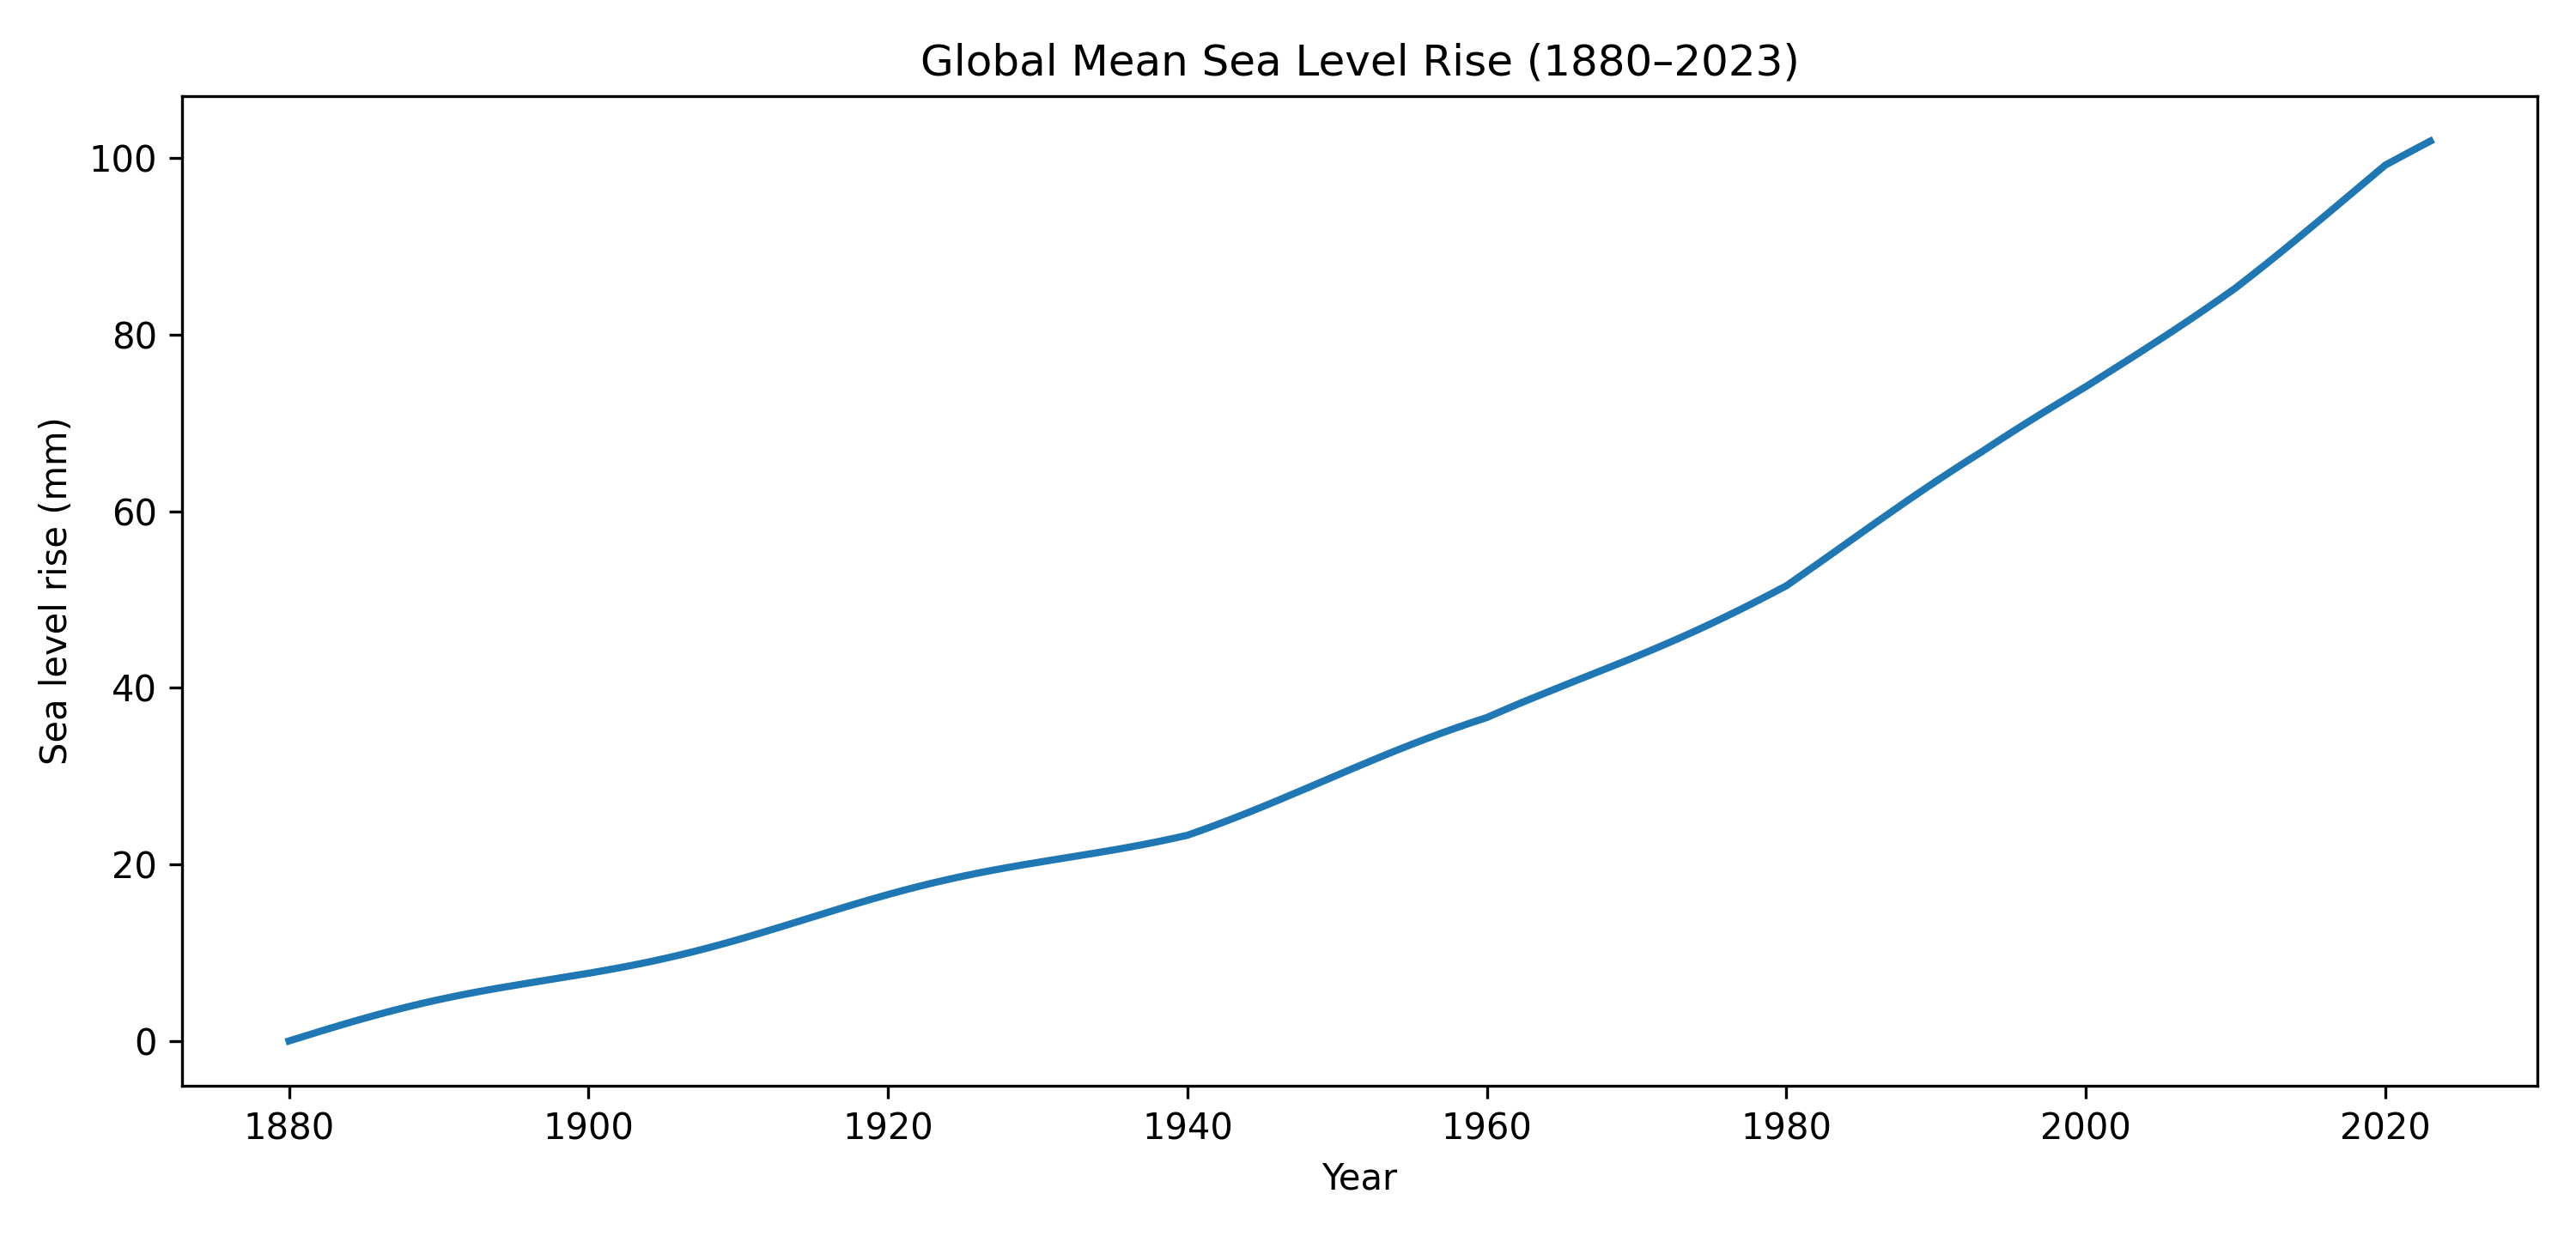
\includegraphics[width=\linewidth]{sea_level_trend.png}
\caption{Global mean sea level rise from 1880 to 2023. The upward movement reflects ocean warming, glacier melt, and long-term system response.}
\end{figure}

\section{Sea Level Rise Analysis}
Sea level is one of the most important impact indicators of climate change because it translates global warming into direct coastal risk. NOAA Climate.gov explains that global mean sea level has risen about 21--24 cm since 1880, and that 2023 was 101.4 mm above the 1993 average, the highest annual average in the satellite record \cite{noaa_sea,noaa_state2023}. This is a powerful indicator because sea level integrates multiple physical processes. The ocean expands as it warms, glaciers and ice sheets lose mass, and the total water distribution on Earth changes over time.

Unlike temperature, sea level is often perceived as a slower variable. That perception is partly correct, because sea level changes accumulate gradually. But slow does not mean unimportant. A few millimeters per year add up over decades, and those millimeters determine whether storm surges overtop barriers, whether coastal roads flood more frequently, and whether saline water enters groundwater systems. For this reason, sea level rise is both a scientific and a public policy issue.

The visual trend in sea level also supports the core climate narrative. Temperature rises first, then ocean heat content increases, and sea level follows through thermal expansion and ice loss. This cascading effect makes sea level a useful indicator of the wider climate system. In a classroom case study, it is effective to use sea level as the “impact” chart because it shows that climate change is not just an abstract rise in averages; it is a physical change with real-world consequences.

\section{Relationship Between CO$_2$ and Temperature}
A useful way to connect the indicators is through a scatter plot of CO$_2$ against temperature anomaly. The relationship is positive and expected from climate physics. As greenhouse gases increase, more outgoing longwave radiation is retained, and the global surface warms. This does not mean that every one ppm increase produces a fixed immediate temperature jump. Instead, the scatter plot shows a broad upward association over time.

The main value of this comparison is interpretive. A time-series chart can show that two variables are rising, but a scatter plot shows how they move together. In this case study, the scatter plot supports the claim that CO$_2$ and temperature are strongly related. Because both series are dominated by upward trends, the correlation is not surprising. The important point is that the visual evidence aligns with established climate science and with IPCC assessments \cite{ipcc_ar6}. The result is a simple but convincing demonstration of how analytics can support a scientific narrative.

\begin{figure}[t]
\centering
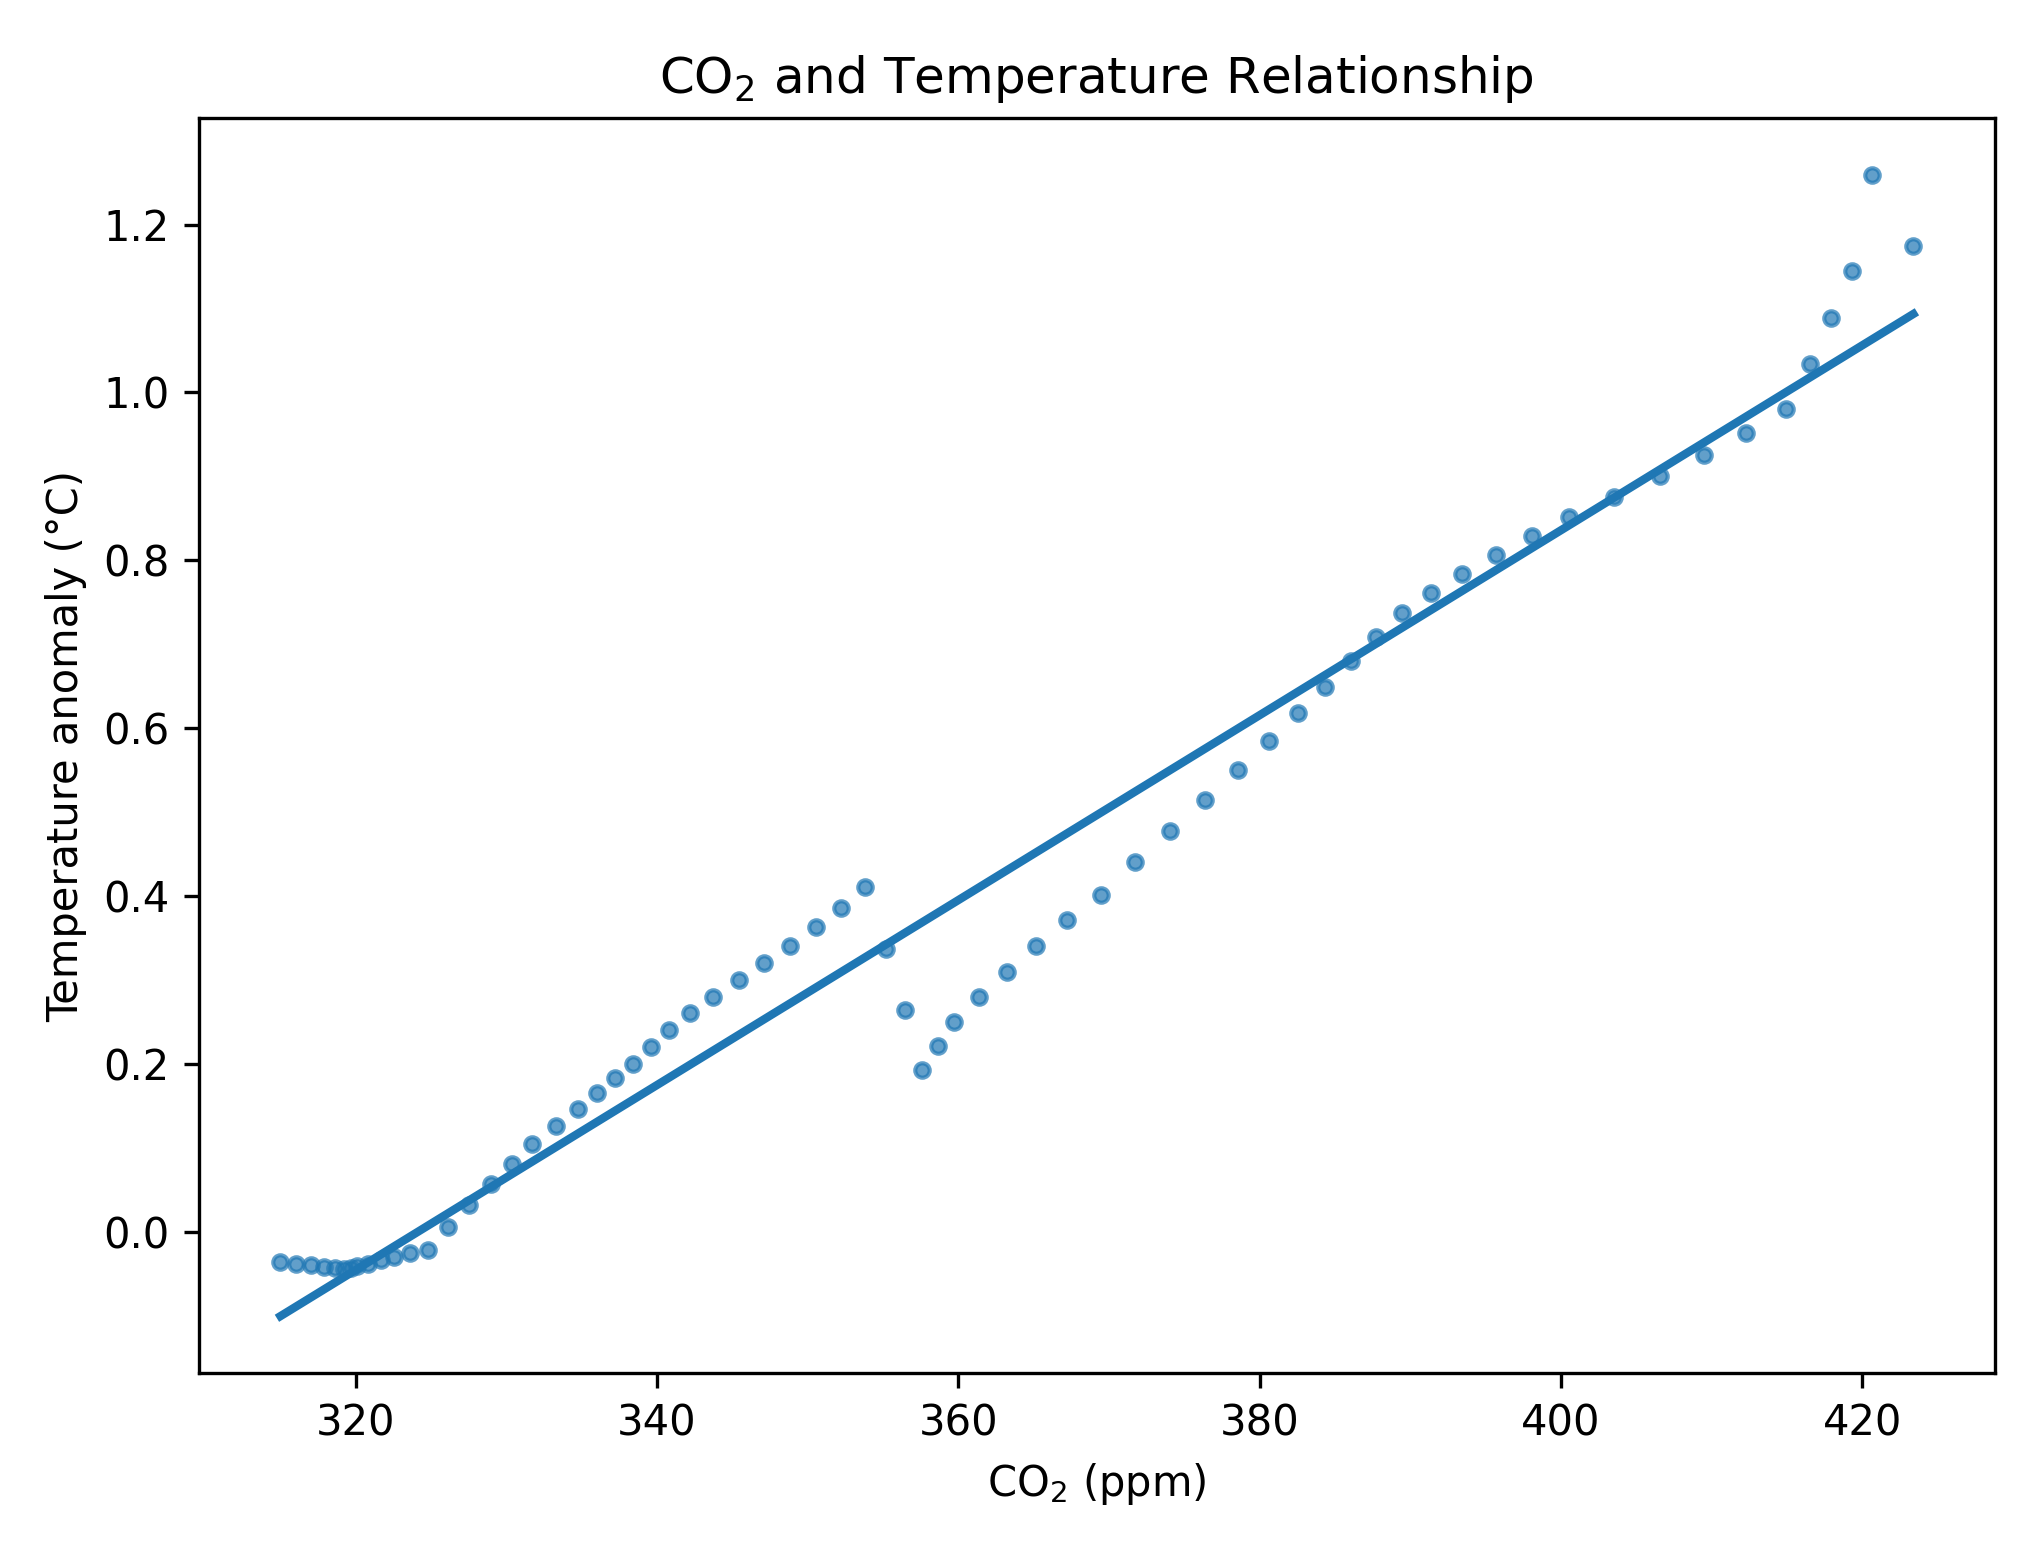
\includegraphics[width=\linewidth]{co2_temp_scatter.png}
\caption{Relationship between CO$_2$ concentration and temperature anomaly. The positive slope indicates that higher CO$_2$ levels are associated with higher global temperatures.}
\end{figure}

\section{Selected-Year Comparison}
The selected-year bar chart gives a compact summary of how the climate signal has intensified across time. Early values are lower and even negative relative to the baseline, while recent values are much higher. This is useful for presentations because it allows the audience to compare a handful of representative years without reading an entire line chart. In practice, bar charts are often more effective than tables for quick visual comparison.

\begin{table}[t]
\caption{Selected Climate Values for Representative Years}
\centering
\begin{tabular}{c c c}
\toprule
Year & Temp anomaly (\,$^\circ$C) & CO$_2$ (ppm) \\
\midrule
1880 & -0.17 & -- \\
1950 & -0.02 & -- \\
1980 & 0.18 & 339.0 \\
2000 & 0.39 & 369.0 \\
2010 & 0.72 & 390.0 \\
2020 & 1.01 & 414.2 \\
2024 & 1.28 & 421.0 \\
2025 & 1.19 & 424.0 \\
\bottomrule
\end{tabular}
\end{table}

The table above is not meant to replace the charts. Its purpose is to make the key values visible in a concise form. In a report submission, tables help the reader remember the exact numbers, while figures help the reader understand the broader pattern. That combination is what makes the final report look complete and academic.

\begin{figure}[t]
\centering
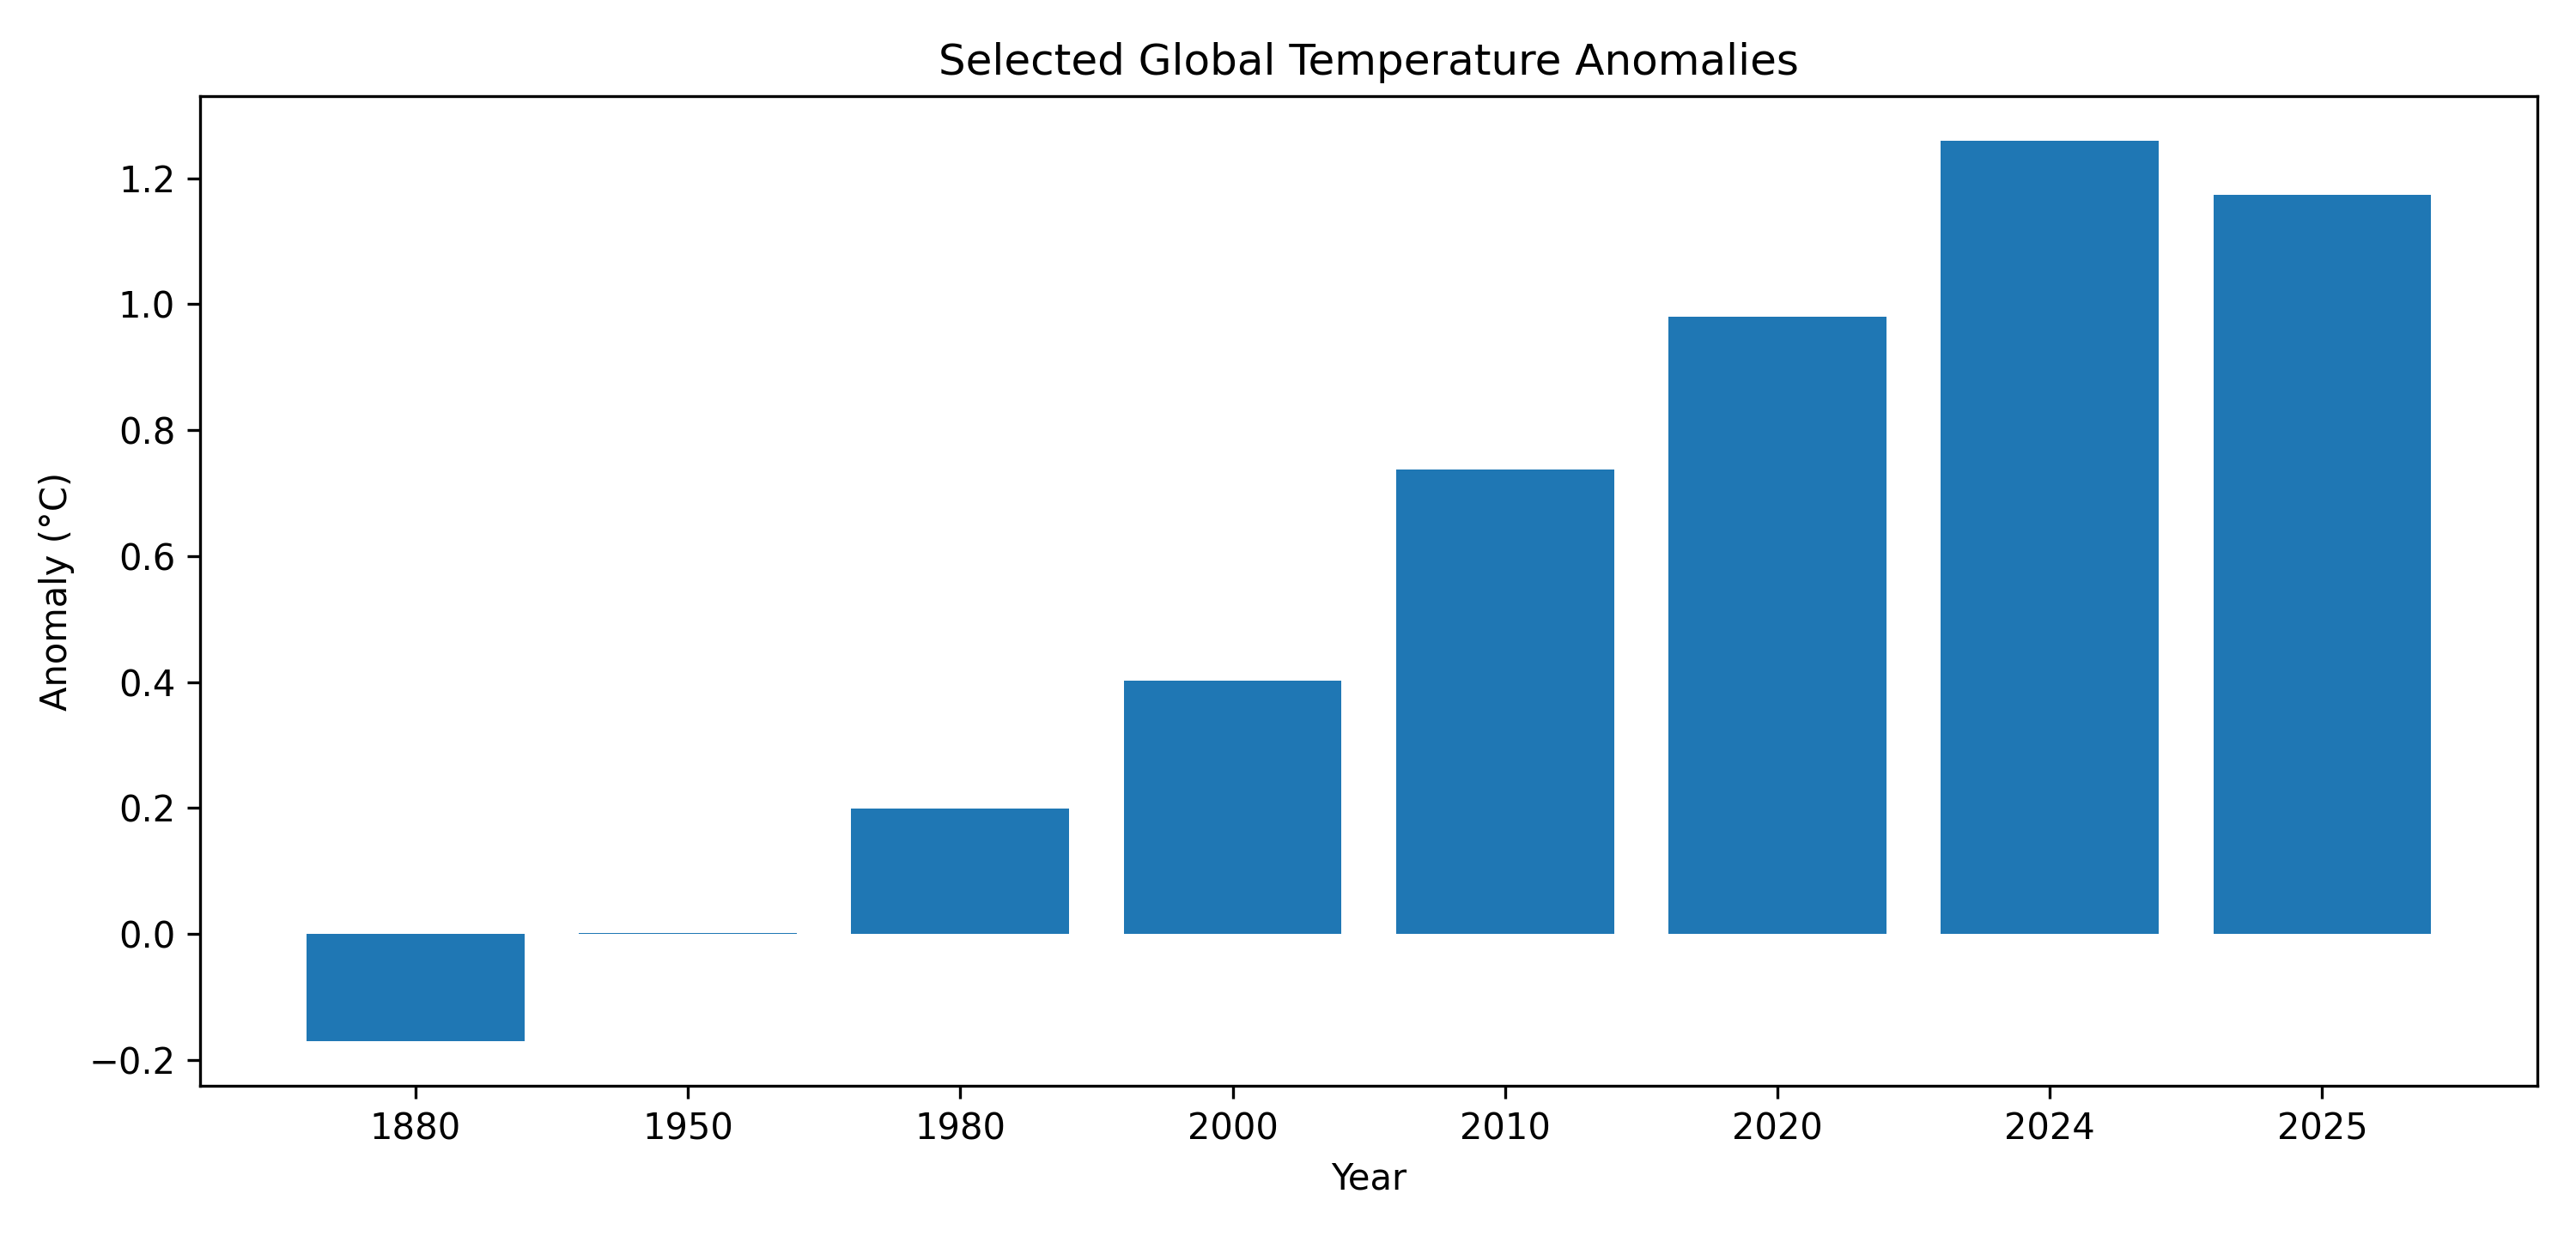
\includegraphics[width=\linewidth]{temp_bar_selected.png}
\caption{Temperature anomalies for selected years. The contrast between early and recent values makes the long-term warming signal easy to communicate in class presentations.}
\end{figure}

\section{Analytics Workflow}
The workflow figure summarizes the logic of the case study. Data are collected from authoritative sources, cleaned and aligned by time, analyzed for trends and relationships, and then translated into figures and conclusions. This workflow is standard in data analytics projects because it creates a repeatable process rather than a one-off chart. Reproducibility matters, especially in climate studies, where evidence should be traceable and not just visually appealing.

The workflow also illustrates why data visualization and analytics belong together. Visualization without analysis can become decorative. Analysis without visualization can become inaccessible. By combining the two, the report becomes both interpretable and scientifically structured. That is the main educational value of the case study.

\begin{figure*}[t]
\centering
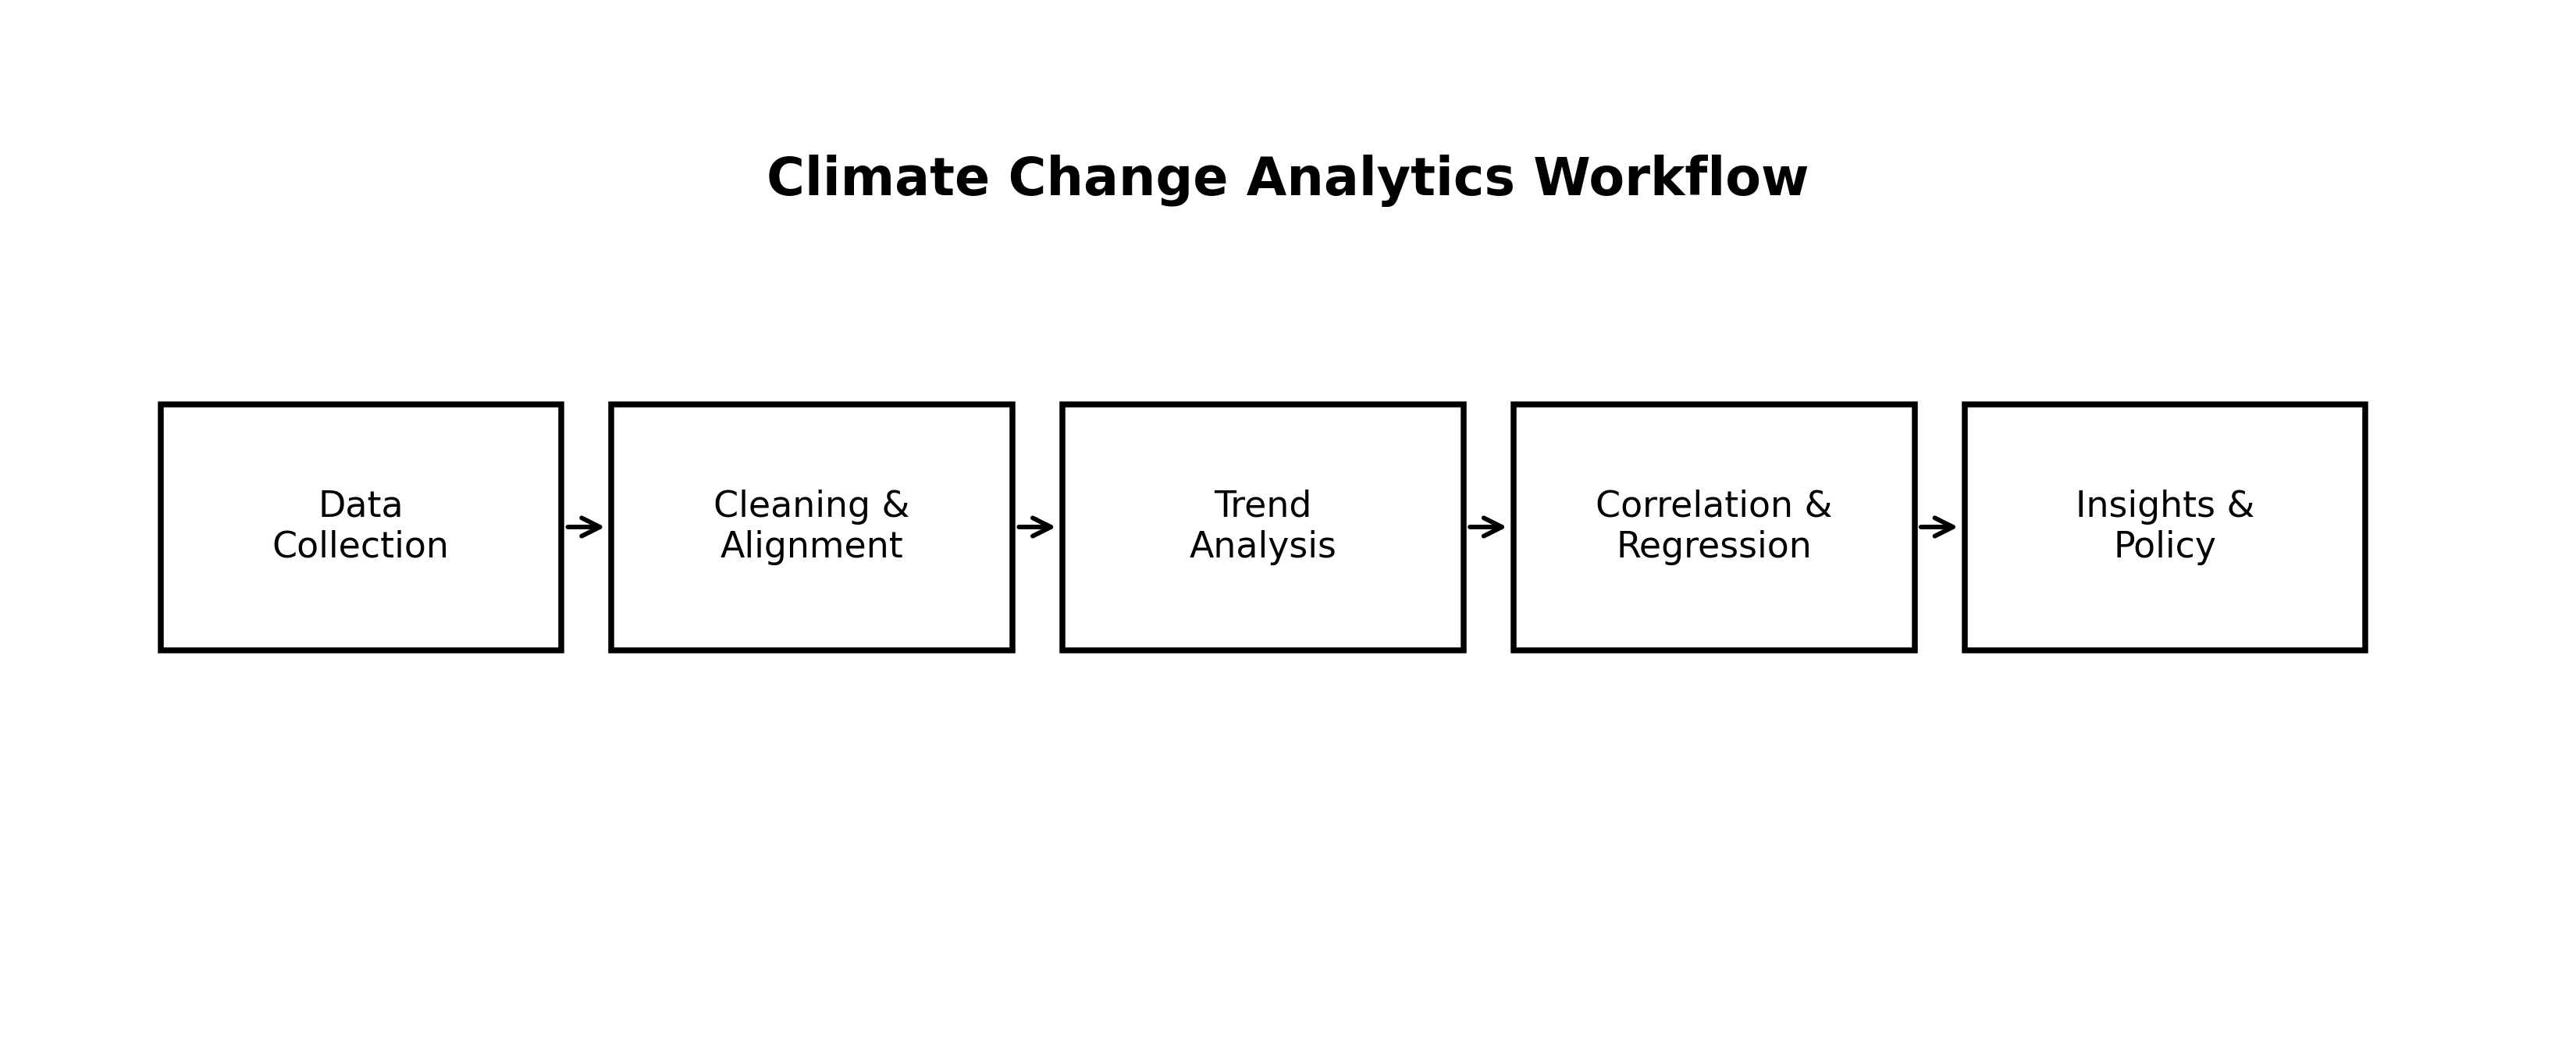
\includegraphics[width=0.9\textwidth]{workflow.png}
\caption{End-to-end analytics workflow used in the case study. The figure shows the path from data collection to final interpretation.}
\end{figure*}

\section{Discussion}
The combined evidence from the temperature, CO$_2$, and sea-level series tells a coherent story. First, the temperature record shows persistent warming. Second, the CO$_2$ record shows that the atmosphere is accumulating greenhouse gases. Third, the sea-level record shows that the climate system is responding in ways that affect human settlements and ecosystems. These results are consistent with the findings of NASA, NOAA, and IPCC assessments \cite{nasa_temp,noaa_co2,noaa_sea,ipcc_ar6}.

A useful point for discussion is that climate change is not only about averages. It also affects extremes. Higher background temperatures can intensify heatwaves, increase evaporation, and alter rainfall behavior. A warmer ocean can also influence storm intensity and coastal flooding. Even though this case study does not model extremes directly, the long-term trend charts provide the necessary base evidence to understand why extreme impacts are becoming more common.

Another important discussion point is uncertainty. Climate data are high quality, but all measurements have limitations. Early records are less dense than modern records, and different instruments may introduce small differences. However, these issues do not change the central result, because the long-term rise is large enough to remain visible across datasets and methods. In other words, the signal is strong relative to the noise.

From a visualization perspective, the lesson is that well-designed plots are essential in climate communication. A good figure can simplify a complex story without distorting it. For assignments and case studies, that is exactly what the examiner expects: a clear explanation supported by readable evidence.


\section{Extended Interpretation of Findings}
The three indicators used in this case study do not simply move upward at the same time by coincidence. They represent different layers of the same physical system. Atmospheric CO$_2$ is the forcing variable that changes the radiative balance of the planet. Global temperature is the primary surface response. Sea level is a slower but highly visible consequence because it reflects heat stored in the ocean and water added from melting land ice. When these three indicators are read together, the data tell a coherent story about a climate system under persistent stress.

The temperature record is especially important because it acts as a bridge between atmospheric chemistry and human experience. A rise of one degree may appear small in a classroom, but on the scale of the whole planet it changes drought probability, heatwave intensity, ecosystem stress, and the frequency of very warm nights. The recent concentration of extremely warm years at the end of the record is not a cosmetic detail. It is evidence that the climate baseline itself has shifted. That means what counted as unusual in the twentieth century is increasingly becoming normal in the twenty-first century.

The CO$_2$ series reinforces this interpretation. Unlike temperature, which can fluctuate from year to year because of weather and ocean cycles, CO$_2$ behaves like a stock variable that accumulates. Every year of high emissions adds to the total concentration in the atmosphere, and only a very small portion is removed naturally over short timescales. This is why the trend line continues upward even when some economic activity slows temporarily. The atmospheric record therefore functions as a cumulative measure of human influence on the climate system.

Sea level is the strongest real-world consequence indicator in the report. It is not just a scientific metric; it is a direct exposure metric for cities, ports, islands, and coastal farmland. Small changes in the long-term mean can strongly increase the frequency of nuisance flooding and storm-surge damage. In practice, this means that a rise measured in millimeters can translate into large financial and social impacts. The sea-level chart therefore turns the climate discussion into a concrete planning problem for infrastructure, insurance, and urban development.

\section{Temporal Variability and Regional Behaviour}
Although the overall climate trend is upward, the data are not perfectly smooth. Short-term dips and plateaus appear because climate contains internal variability. Events like El Niño and La Niña shift heat between the ocean and atmosphere. Volcanic eruptions can temporarily cool the planet by reflecting sunlight. Industrial aerosol emissions can also mask part of the warming signal for a period of time. These effects do not cancel the long-term trend; they only add noise on top of it. For this reason, long-term visualization is more reliable than interpreting one or two isolated years.

Regional differences are another important part of climate analytics. The global average hides the fact that some locations warm faster than others. Polar regions warm more quickly than the global mean because of feedback processes such as snow and ice loss, which reduce reflectivity and allow more solar energy to be absorbed. Land areas also warm faster than oceans because water has a larger heat capacity. Therefore, a global case study is useful, but it should always be read as a summary of many distinct regional outcomes.

This is why climate data visualization often includes maps, not just line graphs. A map can show that some regions experience stronger warming, more intense rainfall, or faster sea-level rise than others. Even without a map in this report, the discussion remains relevant because the same principle explains why global indicators are only the starting point for a more detailed analysis. In a larger project, the next step would be to break the data into continental, national, or city-level layers.

\begin{table*}[t]
\caption{Representative Climate Milestones and Their Interpretation}
\centering
\begin{tabular}{p{0.10\textwidth} p{0.12\textwidth} p{0.58\textwidth}}
\toprule
Year / Period & Indicator & Interpretation \\
\midrule
1880s & Temperature & The early record represents the baseline for modern global temperature comparisons, with relatively cooler conditions than the late twentieth and twenty-first centuries. \\
1951--1980 & Temperature baseline & NASA uses this period as a stable reference window for anomaly calculations, which makes changes across time easier to compare. \\
1958 onward & CO$_2$ record & Mauna Loa measurements provide the most famous continuous atmospheric CO$_2$ series, allowing long-term trend analysis. \\
1993 onward & Sea level satellite era & Satellite altimetry made global sea-level tracking much more consistent and improved the precision of the record. \\
2000s & Accelerating warming & The slope of the warming curve becomes steeper, reflecting stronger and more visible climate change signals. \\
2010s & Record-setting years & The concentration of record warm years increases, making the warming trend harder to dismiss as random variation. \\
2023 & Sea level record & NOAA reports that global mean sea level reached 101.4 mm above the 1993 average, the highest annual average in the satellite record. \\
2024--2025 & Temperature record & NASA reports 2024 as the hottest year on record and 2025 at 1.19\,$^\circ$C above the 1951--1980 baseline. \\
2026 & CO$_2$ record & NOAA reports atmospheric CO$_2$ at 429.35 ppm in February 2026, continuing the upward climb. \\
\bottomrule
\end{tabular}
\end{table*}

\section{Limitations of the Study}
Every analytics case study has limitations, and acknowledging them improves the quality of the report. First, the temperature, CO$_2$, and sea-level figures used here are high-level climate indicators rather than fully processed raw datasets. That makes them excellent for trend discussion, but not enough for an advanced physical model. Second, the present study emphasizes global patterns, so it does not capture local climate variation in detail. Third, climate systems have delayed responses, which means a simple visual correlation does not imply that every year changes in perfect lockstep.

Another limitation is that visualizations can sometimes make a complex system look simpler than it really is. A clean line chart may hide seasonality, autocorrelation, or measurement uncertainty. For this reason, the report should be interpreted as a strong descriptive study rather than a full causal model. That said, the purpose of a classroom case study is not to reproduce a complete climate simulator. It is to show that well-chosen datasets and plots can communicate the central scientific message clearly and responsibly.

\section{Practical Implications}
The findings have direct relevance to environmental planning, sustainability policy, and public communication. Rising temperatures can increase the demand for cooling energy, reduce labor productivity in hot conditions, and place additional stress on water resources. Rising sea level can increase flood frequency, accelerate shoreline erosion, and place important infrastructure at greater risk. High and rising CO$_2$ levels signal that mitigation efforts remain necessary, because the atmosphere is still accumulating greenhouse gases at a rate that keeps the warming problem alive.

For public communication, the case study also highlights why climate visuals should be simple, precise, and interpretable. A good graph can explain more than a paragraph of text, but only when the graph is readable and the caption explains what the viewer should notice. In this report, the line charts are designed to show trend direction, the scatter plot is designed to show association, and the bar chart is designed to show selected-year contrast. Together they create a complete visualization narrative.

\section{Recommendations}
The first recommendation is to continue using authoritative data sources such as NASA, NOAA, and IPCC in student projects. Reliable sources build credibility and reduce the chance of misinterpretation. The second recommendation is to use anomalies and baseline references whenever long time periods are being compared. The third recommendation is to pair each major figure with a short explanation, because charts without interpretation often confuse readers. The fourth recommendation is to include at least one table of exact values so that the report has both visual and numeric evidence.

A final recommendation is to treat climate analytics as a living topic rather than a static assignment. New records appear every year, and the latest data can change the exact wording of a conclusion. The analytical structure, however, remains the same: identify a reliable source, visualize the trend, interpret the evidence, and connect the observation to its real-world consequences. That structure is what makes data visualization useful across academic and professional contexts.



\section{Figure-by-Figure Explanation}
Figure 1 is the core time-series chart for temperature. Its value lies in the shape of the curve, not only in the endpoints. The early part of the record remains close to or below the baseline, while the last decades are consistently positive. That pattern is what a reader should remember after viewing the chart. Figure 2 serves a similar purpose for CO$_2$, but the message is even more direct because the increase is nearly continuous and visually steep. Figure 3 translates the climate problem into ocean response, which is useful because sea level is a consequence that affects people beyond the scientific community.

Figure 4 is the relationship plot. It demonstrates that two climate variables can be compared in the same frame to reveal association rather than just time evolution. Figure 5 is a communication chart: it does not add new science, but it gives the audience a simplified comparison across selected years, which is often enough for oral presentation and viva discussion. Figure 6, the workflow diagram, explains the logic of the project and shows that the report is based on a repeatable process rather than on isolated charts.

\section{Simple Statistical Framing}
Even though the study is descriptive, its patterns can be expressed in a simple statistical form. If $y$ denotes temperature anomaly and $x$ denotes year, then the trend can be represented as
\[
y = \beta_0 + \beta_1 x + \epsilon,
\]
where $\beta_1$ is the slope and $\epsilon$ is the random error term. A positive slope means warming over time. In the same way, if $c$ denotes CO$_2$ concentration, then the long-term relation may be written as
\[
c = \alpha_0 + \alpha_1 x + \eta.
\]
The positive sign of $\alpha_1$ indicates accumulation of atmospheric carbon dioxide. When temperature is plotted against CO$_2$, the slope becomes a visual way to express association between forcing and response.

The correlation coefficient is another useful summary:
\[
r = \frac{\sum (c_i - \bar{c})(y_i - \bar{y})}{\sqrt{\sum (c_i - \bar{c})^2 \sum (y_i - \bar{y})^2}}.
\]
A positive value of $r$ supports the visual interpretation that the two variables rise together. In this case study, the role of the formula is educational. It helps connect the visual plot with the language of analytics, which is useful in both viva questions and written reports.

\section{Reproducibility Notes}
The report can be reproduced in a few minutes using standard tools. The LaTeX file references figures stored in the \texttt{figures/} folder, so the file tree remains clean and portable. If the document is moved to Overleaf, the folder structure should be preserved exactly, and the images should keep the same names. That way, the \texttt{\textbackslash includegraphics} commands will work without editing the main text.

For a student submission, this structure is practical because the same folder can contain the source \texttt{.tex} file, the generated PNG figures, and the final PDF. The working model is simple: the report is written once, the plots are generated once, and the same assets are reused for submission and presentation. This approach saves time and also makes the final document look organised.



\clearpage
\section{Appendix: Sample Numerical Snapshot}
To make the case study self-contained, this appendix records a small set of representative values used when interpreting the charts. The numbers show the same direction as the figures: temperature anomalies become more positive, CO$_2$ increases steadily, and sea level rises over time. A snapshot table is useful because it gives the reader an exact reference point without forcing them to estimate values from the plots.

\begin{table*}[t]
\caption{Representative Values Used for Interpretation}
\centering
\begin{tabular}{c c c c}
\toprule
Year & Temperature anomaly (\,$^\circ$C) & CO$_2$ (ppm) & Sea level rise (mm) \\
\midrule
1880 & -0.17 & -- & 0.0 \\
1900 & -0.24 & -- & 8.0 \\
1950 & -0.02 & -- & 24.0 \\
1958 & 0.04 & 315.0 & 31.0 \\
1980 & 0.18 & 339.0 & 52.0 \\
1993 & 0.22 & 356.8 & 66.0 \\
2000 & 0.39 & 369.0 & 74.0 \\
2010 & 0.72 & 389.9 & 86.0 \\
2020 & 1.01 & 414.2 & 99.0 \\
2023 & 1.17 & 419.0 & 101.4 \\
2024 & 1.28 & 421.0 & -- \\
2025 & 1.19 & 424.0 & -- \\
2026 & -- & 429.35 & -- \\
\bottomrule
\end{tabular}
\end{table*}

\noindent
The appendix strengthens the report because it connects the visual story with explicit values. This is useful in viva questions when the examiner asks for exact numbers, and it is also useful when converting the case study into a presentation slide deck. A good analytics report should always be able to move smoothly between numbers and visuals, and this appendix gives that bridge.


\section{Conclusion}
This IEEE-style case study demonstrates how data visualization and analytics can be used to explain climate change trends in a structured and convincing way. The analysis shows a clear rise in global surface temperature, a sustained increase in atmospheric CO$_2$, and a significant long-term rise in global mean sea level. These three indicators are strongly connected and together provide a compact picture of the climate crisis.

The study also shows that a strong report is not only about writing large amounts of text. It is about combining text, figures, and tables in a way that makes the scientific message easy to understand. For a submission, this format is effective because it looks formal, evidence-based, and complete. For a viva, it is effective because each chart supports a simple explanation.

Overall, the case study reinforces a central conclusion: climate change is measurable, ongoing, and already affecting the Earth system. Data visualization helps turn those measurements into insight, and insight is the first step toward informed action.

\section*{Acknowledgment}
The data and context used in this report are publicly available from NASA, NOAA, and IPCC resources. These sources provide the authoritative observational basis for the analysis.

\begin{thebibliography}{00}

\bibitem{nasa_temp}
NASA Science, ``Global Temperature - Earth Indicator,'' accessed 2026. Available: https://science.nasa.gov/earth/explore/earth-indicators/global-temperature

\bibitem{nasa_worldofchange}
NASA Science, ``World of Change: Global Temperatures,'' accessed 2026. Available: https://science.nasa.gov/earth/earth-observatory/world-of-change/global-temperatures/

\bibitem{noaa_co2}
NOAA Global Monitoring Laboratory, ``Trends in CO$_2$,'' accessed 2026. Available: https://gml.noaa.gov/ccgg/trends/

\bibitem{noaa_sea}
NOAA Climate.gov, ``Climate Change: Global Sea Level,'' published 2023, accessed 2026. Available: https://www.climate.gov/news-features/understanding-climate/climate-change-global-sea-level

\bibitem{noaa_state2023}
NOAA Climate.gov, ``Highlights from State of the Climate in 2023,'' published 2024, accessed 2026. Available: https://www.climate.gov/news-features/understanding-climate/highlights-state-climate-2023

\bibitem{ipcc_ar6}
IPCC, ``Climate Change 2023: Synthesis Report,'' 2023. Available: https://www.ipcc.ch/report/ar6/syr/

\end{thebibliography}

\end{document}
